
\documentclass[12pt,a4paper]{article}
\usepackage{acn-scientific}
\usepackage{acn-questions}
\usepackage[latin1]{inputenc}
\usepackage{amsmath}
\usepackage{amsfonts}
\usepackage{amssymb}
%\usepackage{paracol}
\usepackage[makeroom]{cancel}
\usetikzlibrary{decorations.pathreplacing,
  decorations.markings,
  decorations.pathmorphing}
\usetikzlibrary{arrows,shapes}

\newcommand{\quantlabel}[8][]{\node[text width=#8,fill=#6!40] (#5) at (#7) {the \emph{#2} \par #1 \par unit: \textbf{#3} (\si{#4})};}
\newcommand{\numlabel}[4]{\node[text width=#4,fill=lightgray!40] (#2) at (#3) {#1};}

\setcounter{secnumdepth}{0}
\setlength{\fboxsep}{15pt}

\title{Required formulas for IGCSE Physics (not given)}
\author{\textsc{A.C. Norman}
\\ \href{mailto:ACN.Norman@radley.org.uk}{\texttt{ACN.Norman@radley.org.uk}} }
\date{}

\begin{document}

\maketitle

\tikzstyle{every picture}+=[remember picture]
%  \tikzstyle{na} = [baseline]

\thispagestyle{empty}

\vfill

\begin{enumerate}

\item the relationship between average speed, distance moved and time taken:
\[\text{average speed} = \frac{\text{distance moved}}{\text{time taken}}\]
\framebox{
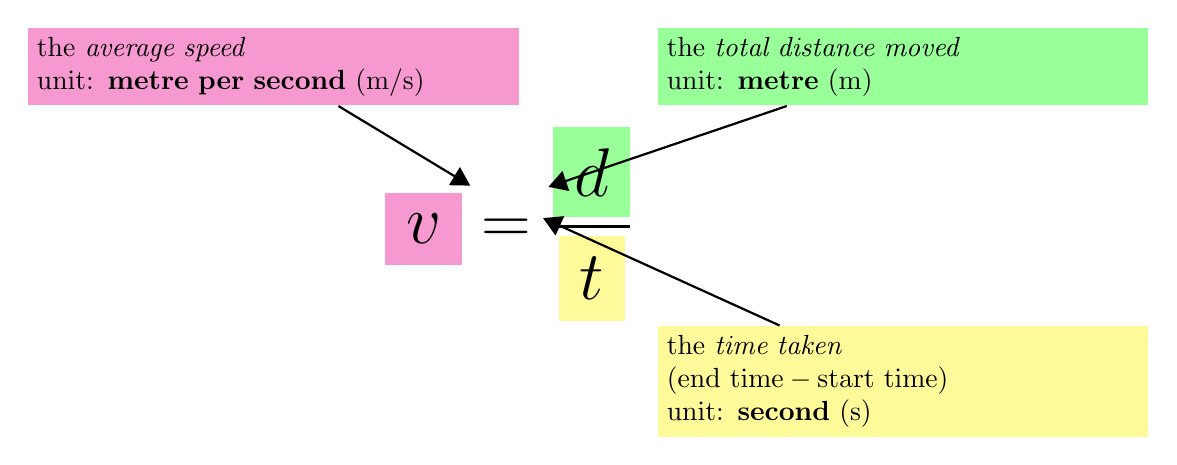
\begin{tikzpicture}[labelpointer/.style={thick, ->, >=triangle 60},]
\quantlabel{average speed}{metre per second}{m/s}{n1}{magenta}{-3,2}{6cm}
\quantlabel[]{total distance moved}{metre}{m}{n2}{green}{5,2}{6cm}
\quantlabel[($\text{end time}-\text{start time}$)]{time taken}{second}{s}{n3}{yellow}{5,-2}{6cm}
\node at (0,0) {\Huge $
  \tikz[baseline]{
    \node[fill=magenta!40,anchor=base] (t1) 
         {$v$};
  }
    =
\dfrac{
    \tikz[baseline]{
      \node[fill=green!40,anchor=base] (t2)
           {$d$};
    } }{
    \tikz[baseline]{
      \node[fill=yellow!40,anchor=base] (t3)
           {$t$};
    }
}
$ };
    \draw[labelpointer] (n1) -- (t1);
    \draw[labelpointer] (n2) -- (t2);
    \draw[labelpointer] (n3) -- (t3);
\end{tikzpicture}
}

\item the relationship between unbalanced force, mass and acceleration:
\[\text{force} = \text{mass} \times \text{acceleration}\]
\framebox{
\begin{tikzpicture}[labelpointer/.style={thick, ->, >=triangle 60},]
\quantlabel{overall force}{newton}{N}{n1}{blue}{-3,2}{4cm}
\quantlabel{mass}{kilogram}{kg}{n2}{red}{-2,-2}{6cm}
\quantlabel[(in direction of resultant force)]{acceleration}{metre per second per second}{m/s^{2}}{n3}{lime}{4.5,2}{8.5cm}
\node at (0,0) {\Huge $
  \tikz[baseline]{
    \node[fill=blue!40,anchor=base] (t1) 
         {$F$};
  }
    =
    \tikz[baseline]{
      \node[fill=red!40,anchor=base] (t2)
           {$m$};
    } \times
    \tikz[baseline]{
      \node[fill=lime!40,anchor=base] (t3)
           {$a$};
    }
$ };
    \draw[labelpointer] (n1) -- (t1);
    \draw[labelpointer] (n2) -- (t2);
    \draw[labelpointer] (n3) -- (t3);
\end{tikzpicture}
}

\newpage

\item the relationship between acceleration, change in velocity and time taken:
\[\text{acceleration} = \frac{\text{change in velocity}}{\text{time}}\]
\framebox{
\begin{tikzpicture}[labelpointer/.style={thick, ->, >=triangle 60},]
\quantlabel{acceleration}{metre per second per second}{m/s^{2}}{n1}{lime}{-1,2}{8.5cm}
\quantlabel[($\text{final speed}-\text{starting speed}$)]{change in speed}{metre per second}{m/s}{n2}{magenta}{5.6,0}{6cm}
\quantlabel[($\text{end time}-\text{start time}$)]{time taken}{second}{s}{n3}{yellow}{5,-2}{6cm}
\node at (0,0) {\Huge $
  \tikz[baseline]{
    \node[fill=lime!40,anchor=base] (t1) 
         {$a$};
  }
    =
\dfrac{
    \tikz[baseline]{
      \node[fill=magenta!40,anchor=base] (t2)
           {$\Delta v$};
    } }{
    \tikz[baseline]{
      \node[fill=yellow!40,anchor=base] (t3)
           {$t$};
    }
}
$ };
    \draw[labelpointer] (n1) -- (t1);
    \draw[labelpointer] (n2) -- (t2);
    \draw[labelpointer] (n3) -- (t3);
\end{tikzpicture}
}

\item the relationship between density, mass and volume:
\[\text{density} = \frac{\text{mass}}{\text{volume}}\]
\framebox{
\begin{tikzpicture}[labelpointer/.style={thick, ->, >=triangle 60},]
\quantlabel{average density}{kilogram per metre cubed}{kg/m^{3}}{n1}{pink}{-3,2}{8.5cm}
\quantlabel{mass}{kilogram}{kg}{n2}{red}{5,1}{4cm}
\quantlabel{volume}{metre cubed}{m^{3}}{n3}{brown}{5,-2}{5cm}
\node at (0,0) {\Huge $
  \tikz[baseline]{
    \node[fill=pink!40,anchor=base] (t1) 
         {$\rho$};
  }
    =
\dfrac{
    \tikz[baseline]{
      \node[fill=red!40,anchor=base] (t2)
           {$m$};
    } }{
    \tikz[baseline]{
      \node[fill=brown!40,anchor=base] (t3)
           {$V$};
    }
}
$ };
    \draw[labelpointer] (n1) -- (t1);
    \draw[labelpointer] (n2) -- (t2);
    \draw[labelpointer] (n3) -- (t3);
\end{tikzpicture}
}

\item the relationship between work done, force and distance moved:
\[\text{work done} = \text{force} \times \text{distance moved}\]
\framebox{
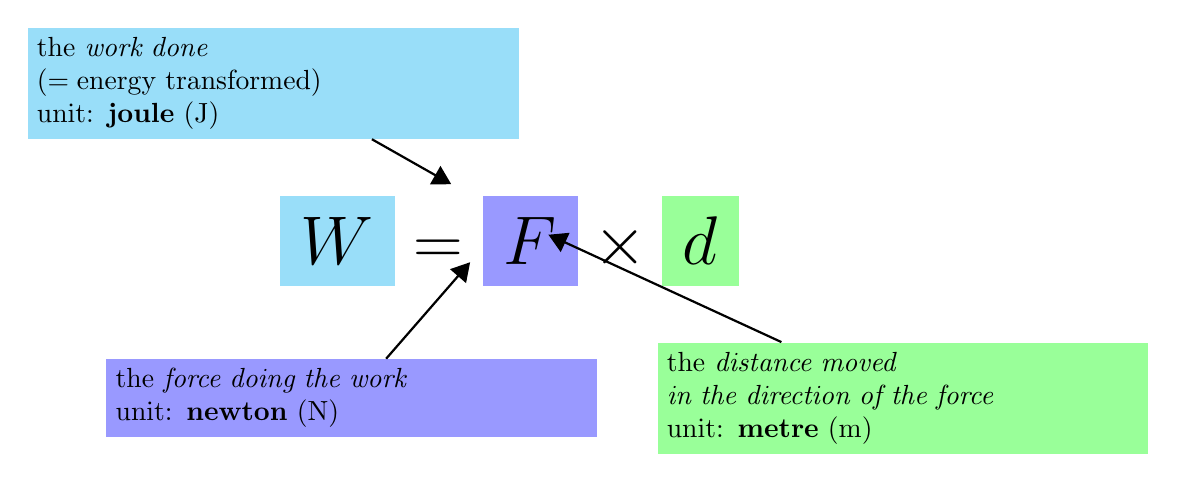
\begin{tikzpicture}[labelpointer/.style={thick, ->, >=triangle 60},]
\quantlabel[($=\text{energy transformed}$)]{work done}{joule}{J}{n1}{cyan}{-3,2}{6cm}
\quantlabel{force doing the work}{newton}{N}{n2}{blue}{-2,-2}{6cm}
\quantlabel[\emph{in the direction of the force}]{distance moved}{metre}{m}{n3}{green}{5,-2}{6cm}
\node at (0,0) {\Huge $
  \tikz[baseline]{
    \node[fill=cyan!40,anchor=base] (t1) 
         {$W$};
  }
    =
    \tikz[baseline]{
      \node[fill=blue!40,anchor=base] (t2)
           {$F$};
    } \times
    \tikz[baseline]{
      \node[fill=green!40,anchor=base] (t3)
           {$d$};
    }
$ };
    \draw[labelpointer] (n1) -- (t1);
    \draw[labelpointer] (n2) -- (t2);
    \draw[labelpointer] (n3) -- (t3);
\end{tikzpicture}
}

\item the energy relationships:
\[\text{energy transferred}=\text{work done}\]
\[\text{kinetic energy}=\frac{1}{2}\times\text{mass}\times\text{speed}^{2}\]
\framebox{
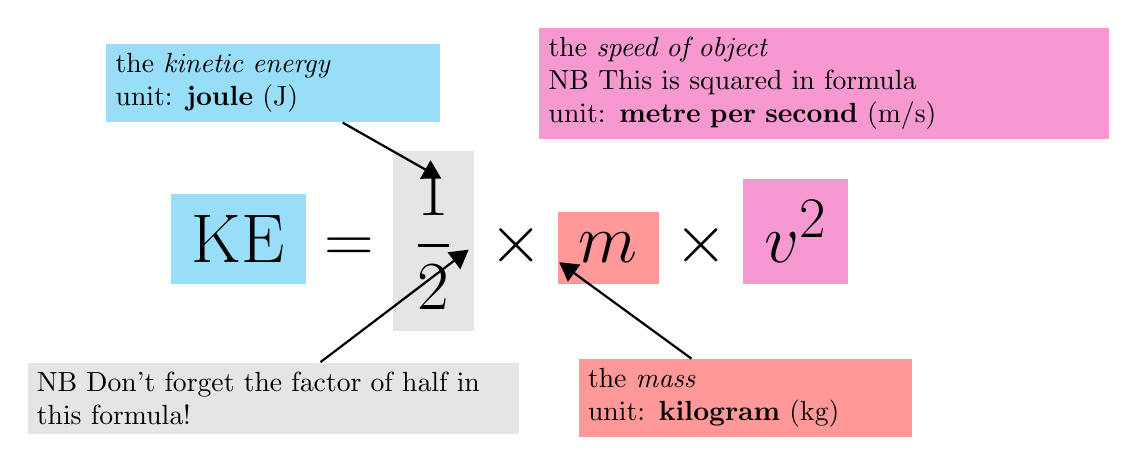
\begin{tikzpicture}[labelpointer/.style={thick, ->, >=triangle 60},]
\quantlabel{kinetic energy}{joule}{J}{n1}{cyan}{-3,2}{4cm}
\numlabel{NB Don't forget the factor of half in this formula!}{n2}{-3,-2}{6cm}
\quantlabel{mass}{kilogram}{kg}{n3}{red}{3,-2}{4cm}
\quantlabel[NB This is squared in formula]{speed of object}{metre per second}{m/s}{n4}{magenta}{4,2}{7cm}

\node at (0,0) {\Huge $
  \tikz[baseline]{
    \node[fill=cyan!40,anchor=base] (t1) 
         {KE};
  } = 
  \tikz[baseline]{
    \node[fill=lightgray!40,anchor=base] (t2) 
         {$\dfrac{1}{2}$};
  } \times
    \tikz[baseline]{
      \node[fill=red!40,anchor=base] (t3)
           {$m$};
    } \times
    \tikz[baseline]{
      \node[fill=magenta!40,anchor=base] (t4)
           {$v^{2}$};
    }
$ };
    \draw[labelpointer] (n1) -- (t1);
    \draw[labelpointer] (n2) -- (t2);
    \draw[labelpointer] (n3) -- (t3);
%    \draw[labelpointer] (n4) -- (t4);
\end{tikzpicture}
}

\[\text{gravitational potential energy}=\text{mass}\times g \times\text{height}\]
\framebox{
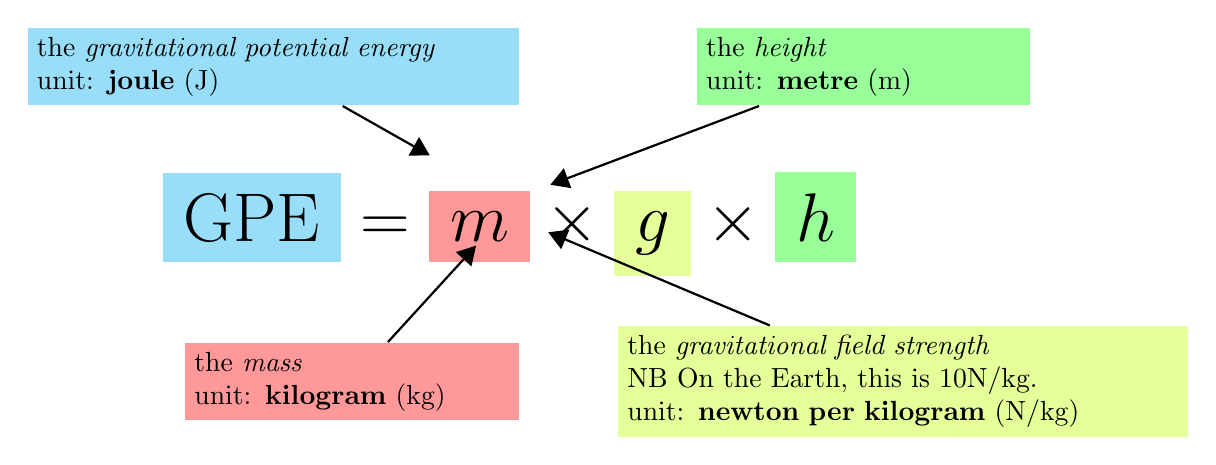
\begin{tikzpicture}[labelpointer/.style={thick, ->, >=triangle 60},]
\quantlabel{gravitational potential energy}{joule}{J}{n1}{cyan}{-3,2}{6cm}
\quantlabel{mass}{kilogram}{kg}{n2}{red}{-2,-2}{4cm}
\quantlabel[NB On the Earth, this is \SI{10}{N/kg}.]{gravitational field strength}{newton per kilogram}{N/kg}{n3}{lime}{5,-2}{7cm}
\quantlabel{height}{metre}{m}{n4}{green}{4.5,2}{4cm}
\node at (0,0) {\Huge $
  \tikz[baseline]{
    \node[fill=cyan!40,anchor=base] (t1) 
         {GPE};
  }
    =
    \tikz[baseline]{
      \node[fill=red!40,anchor=base] (t2)
           {$m$};
    } \times
    \tikz[baseline]{
      \node[fill=lime!40,anchor=base] (t3)
           {$g$};
    } \times
    \tikz[baseline]{
      \node[fill=green!40,anchor=base] (t4)
           {$h$};
    }
$ };
    \draw[labelpointer] (n1) -- (t1);
    \draw[labelpointer] (n2) -- (t2);
    \draw[labelpointer] (n3) -- (t3);
    \draw[labelpointer] (n4) -- (t4);
\end{tikzpicture}
}

\item the relationship between weight, mass and gravitational field strength:
\[\text{weight}=\text{mass}\times\text{gravitational field strength}\]
\framebox{
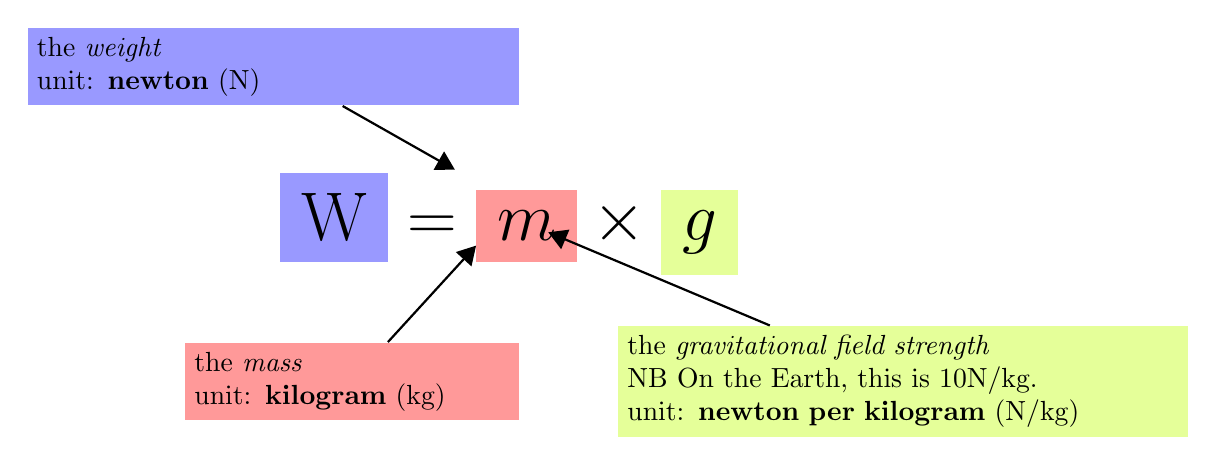
\begin{tikzpicture}[labelpointer/.style={thick, ->, >=triangle 60},]
\quantlabel{weight}{newton}{N}{n1}{blue}{-3,2}{6cm}
\quantlabel{mass}{kilogram}{kg}{n2}{red}{-2,-2}{4cm}
\quantlabel[NB On the Earth, this is \SI{10}{N/kg}.]{gravitational field strength}{newton per kilogram}{N/kg}{n3}{lime}{5,-2}{7cm}
\node at (0,0) {\Huge $
  \tikz[baseline]{
    \node[fill=blue!40,anchor=base] (t1) 
         {W};
  }
    =
    \tikz[baseline]{
      \node[fill=red!40,anchor=base] (t2)
           {$m$};
    } \times
    \tikz[baseline]{
      \node[fill=lime!40,anchor=base] (t3)
           {$g$};
    } 
$ };
    \draw[labelpointer] (n1) -- (t1);
    \draw[labelpointer] (n2) -- (t2);
    \draw[labelpointer] (n3) -- (t3);
\end{tikzpicture}
}

\item the relationship between pressure, force and area:
\[\text{pressure} = \frac{\text{force}}{\text{area}}\]
\framebox{
\begin{tikzpicture}[labelpointer/.style={thick, ->, >=triangle 60},]
\quantlabel{resulting pressure}{pascal}{Pa}{n1}{blue!20!}{-3,2}{4cm}
\quantlabel{applied force}{newton}{N}{n2}{blue}{5,1}{4cm}
\quantlabel{area \emph{over which it acts}}{metre squared}{m^{2}}{n3}{orange}{5,-2}{5cm}
\node at (0,0) {\Huge $
  \tikz[baseline]{
    \node[fill=blue!20!!40,anchor=base] (t1) 
         {$p$};
  }
    =
\dfrac{
    \tikz[baseline]{
      \node[fill=blue!40,anchor=base] (t2)
           {$F$};
    } }{
    \tikz[baseline]{
      \node[fill=orange!40,anchor=base] (t3)
           {$A$};
    }
}
$ };
    \draw[labelpointer] (n1) -- (t1);
    \draw[labelpointer] (n2) -- (t2);
    \draw[labelpointer] (n3) -- (t3);
\end{tikzpicture}
}

\item the relationship between charge, current, voltage, resistance and electrical power:
\[\text{charge}=\text{current}\times\text{time}\]
\framebox{
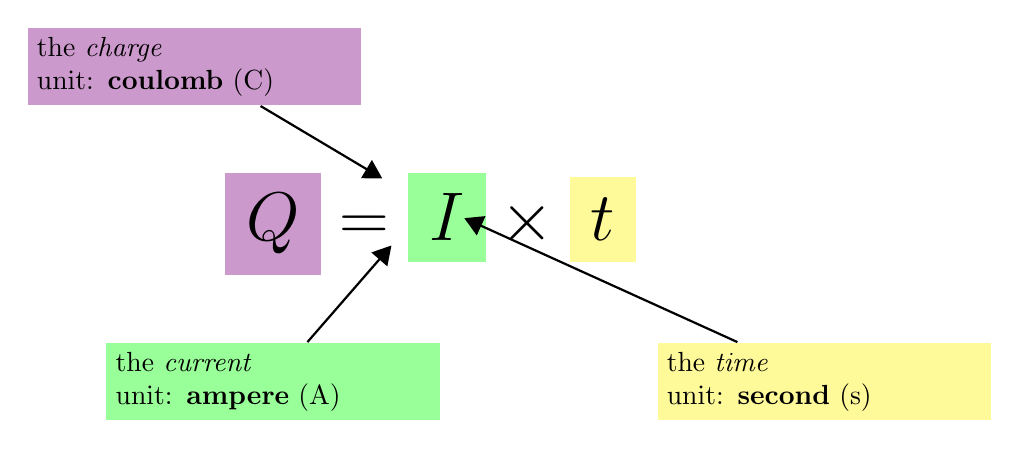
\begin{tikzpicture}[labelpointer/.style={thick, ->, >=triangle 60},]
\quantlabel{charge}{coulomb}{C}{n1}{violet}{-3,2}{4cm}
\quantlabel{current}{ampere}{A}{n2}{green}{-2,-2}{4cm}
\quantlabel{time}{second}{s}{n3}{yellow}{5,-2}{4cm}
\node at (0,0) {\Huge $
  \tikz[baseline]{
    \node[fill=violet!40,anchor=base] (t1) 
         {$Q$};
  }
    =
    \tikz[baseline]{
      \node[fill=green!40,anchor=base] (t2)
           {$I$};
    } \times
    \tikz[baseline]{
      \node[fill=yellow!40,anchor=base] (t3)
           {$t$};
    } 
$ };
    \draw[labelpointer] (n1) -- (t1);
    \draw[labelpointer] (n2) -- (t2);
    \draw[labelpointer] (n3) -- (t3);
\end{tikzpicture}
}

\[\text{voltage}=\text{current}\times\text{resistance}\]
\framebox{
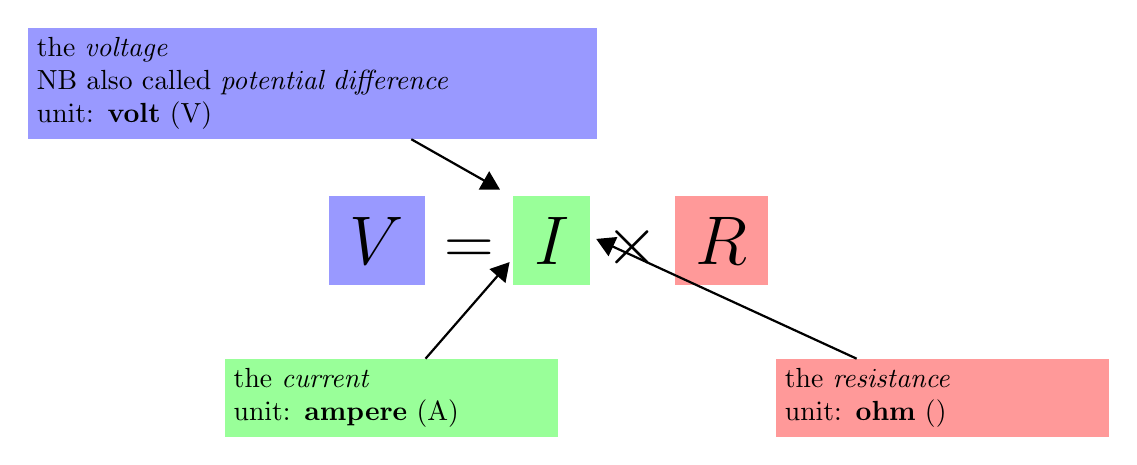
\begin{tikzpicture}[labelpointer/.style={thick, ->, >=triangle 60},]
\quantlabel[NB also called \emph{potential difference}]{voltage}{volt}{V}{n1}{blue}{-3,2}{7cm}
\quantlabel{current}{ampere}{A}{n2}{green}{-2,-2}{4cm}
\quantlabel{resistance}{ohm}{\ohm}{n3}{red}{5,-2}{4cm}
\node at (0,0) {\Huge $
  \tikz[baseline]{
    \node[fill=blue!40,anchor=base] (t1) 
         {$V$};
  }
    =
    \tikz[baseline]{
      \node[fill=green!40,anchor=base] (t2)
           {$I$};
    } \times
    \tikz[baseline]{
      \node[fill=red!40,anchor=base] (t3)
           {$R$};
    } 
$ };
    \draw[labelpointer] (n1) -- (t1);
    \draw[labelpointer] (n2) -- (t2);
    \draw[labelpointer] (n3) -- (t3);
\end{tikzpicture}
}

\[\text{electrical power}=\text{voltage}\times\text{current}\]
\framebox{
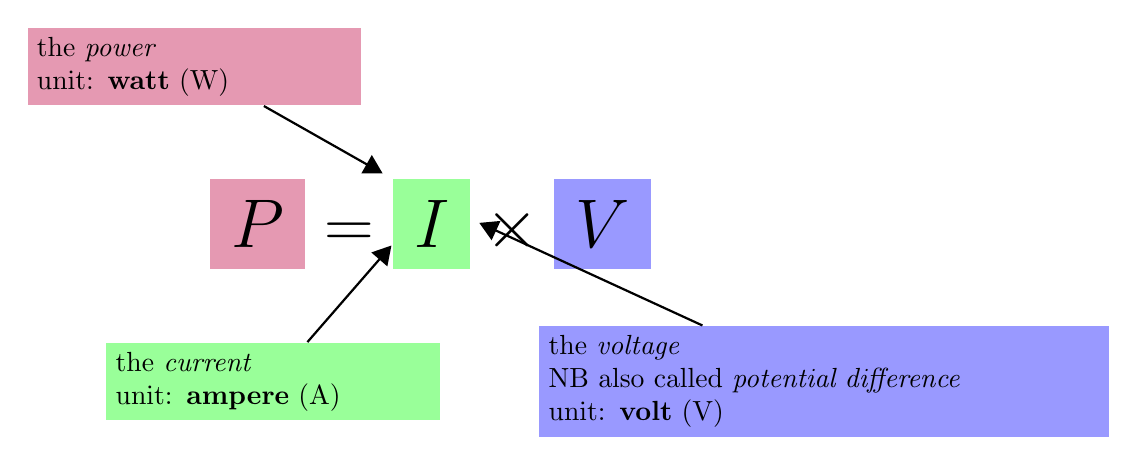
\begin{tikzpicture}[labelpointer/.style={thick, ->, >=triangle 60},]
\quantlabel{power}{watt}{W}{n1}{purple}{-3,2}{4cm}
\quantlabel{current}{ampere}{A}{n2}{green}{-2,-2}{4cm}
\quantlabel[NB also called \emph{potential difference}]{voltage}{volt}{V}{n3}{blue}{5,-2}{7cm}
\node at (0,0) {\Huge $
  \tikz[baseline]{
    \node[fill=purple!40,anchor=base] (t1) 
         {$P$};
  }
    =
    \tikz[baseline]{
      \node[fill=green!40,anchor=base] (t2)
           {$I$};
    } \times
    \tikz[baseline]{
      \node[fill=blue!40,anchor=base] (t3)
           {$V$};
    } 
$ };
    \draw[labelpointer] (n1) -- (t1);
    \draw[labelpointer] (n2) -- (t2);
    \draw[labelpointer] (n3) -- (t3);
\end{tikzpicture}
}

\item the relationship between energy transferred, charge and voltage:
\[\text{energy transferred}=\text{charge}\times\text{voltage}\]
\framebox{
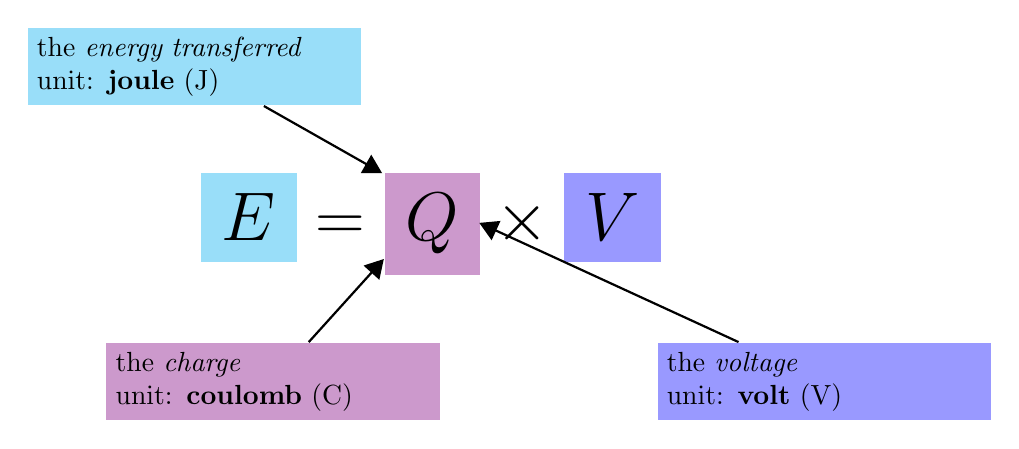
\begin{tikzpicture}[labelpointer/.style={thick, ->, >=triangle 60},]
\quantlabel{energy transferred}{joule}{J}{n1}{cyan}{-3,2}{4cm}
\quantlabel{charge}{coulomb}{C}{n2}{violet}{-2,-2}{4cm}
\quantlabel{voltage}{volt}{V}{n3}{blue}{5,-2}{4cm}
\node at (0,0) {\Huge $
  \tikz[baseline]{
    \node[fill=cyan!40,anchor=base] (t1) 
         {$E$};
  }
    =
    \tikz[baseline]{
      \node[fill=violet!40,anchor=base] (t2)
           {$Q$};
    } \times
    \tikz[baseline]{
      \node[fill=blue!40,anchor=base] (t3)
           {$V$};
    } 
$ };
    \draw[labelpointer] (n1) -- (t1);
    \draw[labelpointer] (n2) -- (t2);
    \draw[labelpointer] (n3) -- (t3);
\end{tikzpicture}
}


\item the relationship between the speed, frequency and wavelength of a wave:
\[\text{wave speed} = \text{frequency} \times \text{wavelength}\]
\framebox{
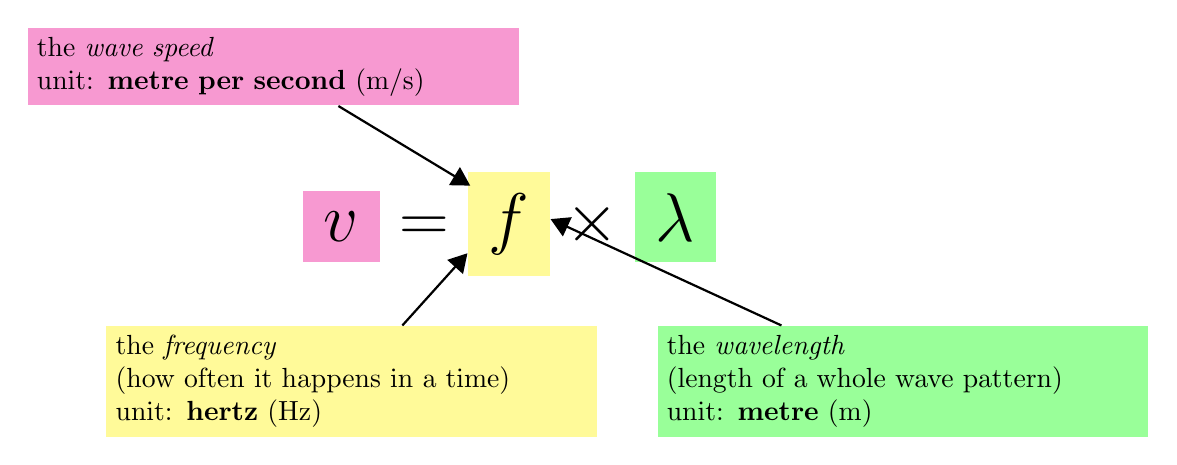
\begin{tikzpicture}[labelpointer/.style={thick, ->, >=triangle 60},]
\quantlabel{wave speed}{metre per second}{m/s}{n1}{magenta}{-3,2}{6cm}
\quantlabel[(how often it happens in a time)]{frequency}{hertz}{Hz}{n2}{yellow}{-2,-2}{6cm}
\quantlabel[(length of a whole wave pattern)]{wavelength}{metre}{m}{n3}{green}{5,-2}{6cm}
\node at (0,0) {\Huge $
  \tikz[baseline]{
    \node[fill=magenta!40,anchor=base] (t1) 
         {$v$};
  }
    =
    \tikz[baseline]{
      \node[fill=yellow!40,anchor=base] (t2)
           {$f$};
    } \times
    \tikz[baseline]{
      \node[fill=green!40,anchor=base] (t3)
           {$\lambda$};
    }
$ };
    \draw[labelpointer] (n1) -- (t1);
    \draw[labelpointer] (n2) -- (t2);
    \draw[labelpointer] (n3) -- (t3);
\end{tikzpicture}
}

\item the relationship between refractive index, angle of incidence and angle of refraction:
\[n=\frac{\sin i}{\sin r}\]
\framebox{
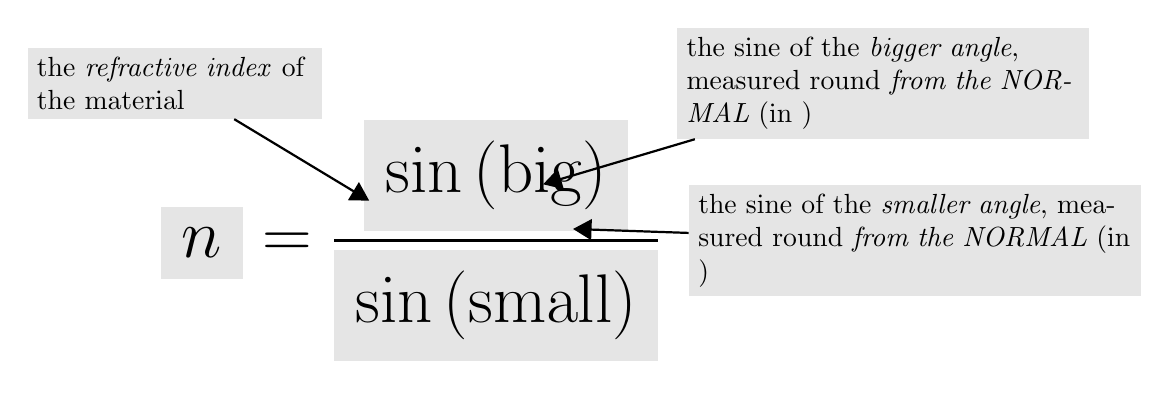
\begin{tikzpicture}[labelpointer/.style={thick, ->, >=triangle 60},]
\numlabel{the \emph{refractive index} of the material}{n1}{-3,2}{3.5cm}
\numlabel{the sine of the \emph{bigger angle}, measured round \emph{from the NORMAL} (in \si{\degree})}{n2}{6,2}{5cm}
\numlabel{the sine of the \emph{smaller angle}, measured round \emph{from the NORMAL} (in \si{\degree})}{n3}{6.4,0}{5.5cm}
\node at (0,0) {\Huge $
  \tikz[baseline]{
    \node[fill=lightgray!40,anchor=base] (t1) 
         {$n$};
  }
    =
\dfrac{
    \tikz[baseline]{
      \node[fill=lightgray!40,anchor=base] (t2)
           {$\sin\left(\text{big}\right)$};
    } }{
    \tikz[baseline]{
      \node[fill=lightgray!40,anchor=base] (t3)
           {$\sin\left(\text{small}\right)$};
    }
}
$ };
    \draw[labelpointer] (n1) -- (t1);
    \draw[labelpointer] (n2) -- (t2);
    \draw[labelpointer] (n3) -- (t3);
\end{tikzpicture}
}

\vfill

\item the relationship between critical angle and refractive index:
\[\sin c=\frac{1}{n}\]
\framebox{
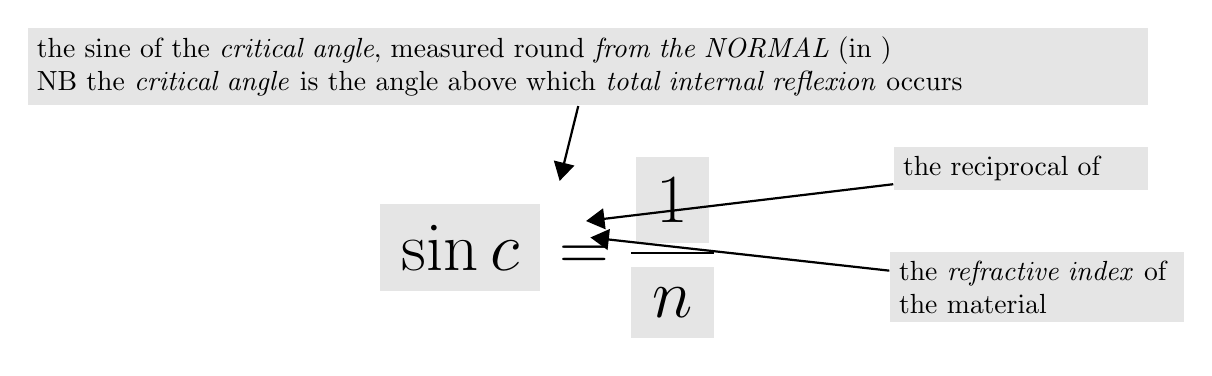
\begin{tikzpicture}[labelpointer/.style={thick, ->, >=triangle 60},]
\numlabel{the sine of the \emph{critical angle}, measured round \emph{from the NORMAL} (in \si{\degree}) \par NB the \emph{critical angle} is the angle above which \emph{total internal reflexion} occurs}{n1}{0.5,2.3}{14cm}
\numlabel{the reciprocal of}{n2}{6,1}{3cm}
\numlabel{the \emph{refractive index} of the material}{n3}{6.2,-0.5}{3.5cm}
\node at (0,0) {\Huge $
  \tikz[baseline]{
    \node[fill=lightgray!40,anchor=base] (t1) 
         {$\sin c$};
  }
    =
\dfrac{
    \tikz[baseline]{
      \node[fill=lightgray!40,anchor=base] (t2)
           {$1$};
    } }{
    \tikz[baseline]{
      \node[fill=lightgray!40,anchor=base] (t3)
           {$n$};
    }
}
$ };
    \draw[labelpointer] (n1) -- (t1);
    \draw[labelpointer] (n2) -- (t2);
    \draw[labelpointer] (n3) -- (t3);
\end{tikzpicture}
}

\vfill

\newpage

\item the relationship for efficiency
\[\text{efficiency} = \frac{\text{useful energy output}}{\text{total energy input}}\times100\% \]
\framebox{
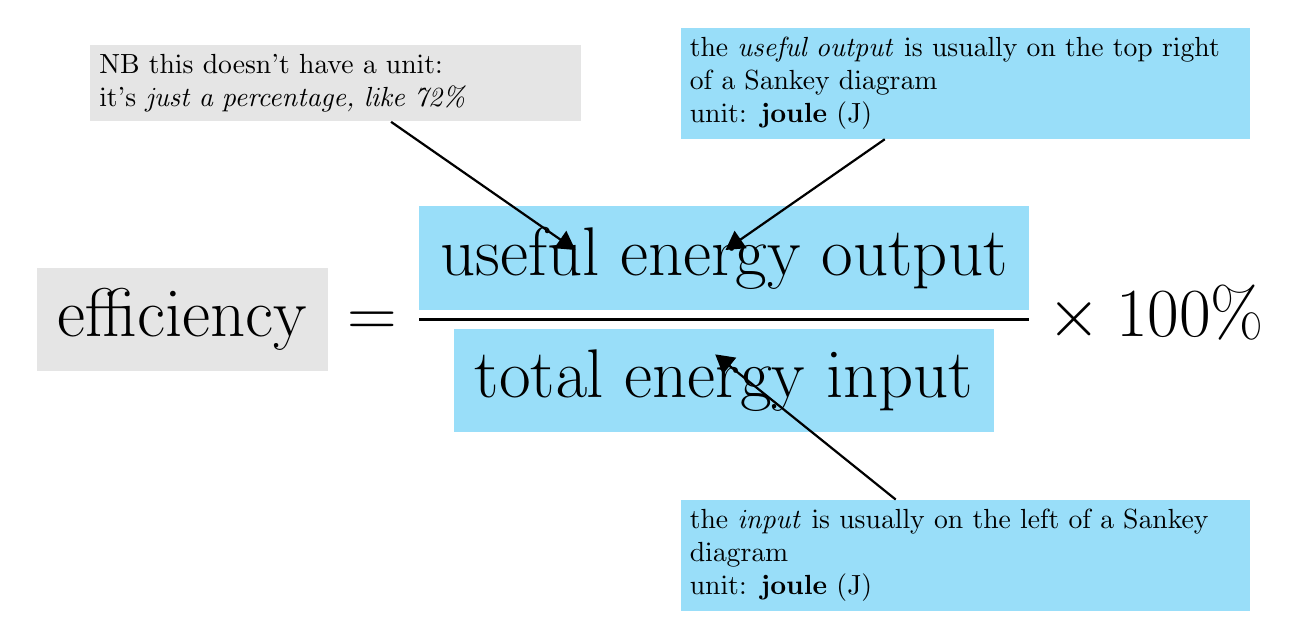
\begin{tikzpicture}[labelpointer/.style={thick, ->, >=triangle 60},]
\numlabel{NB this doesn't have a unit:\\it's \emph{just a percentage, like 72\%}}{n1}{-4,3}{6cm}
\quantlabel[]{useful output \emph{is usually on the top right of a Sankey diagram}}{joule}{J}{n2}{cyan}{4,3}{7cm}
\quantlabel[]{input \emph{is usually on the left of a Sankey diagram}}{joule}{J}{n3}{cyan}{4,-3}{7cm}
\node at (0,0) {\Huge $
  \tikz[baseline]{
    \node[fill=lightgray!40,anchor=base] (t1) 
         {efficiency};
  }
    =
\dfrac{
    \tikz[baseline]{
      \node[fill=cyan!40,anchor=base] (t2)
           {useful energy output};
    } }{
    \tikz[baseline]{
      \node[fill=cyan!40,anchor=base] (t3)
           {total energy input};
    }
} \times 100 \%
$ };
    \draw[labelpointer] (n1) -- (t1);
    \draw[labelpointer] (n2) -- (t2);
    \draw[labelpointer] (n3) -- (t3);
\end{tikzpicture}
}

\item the relationship for pressure difference:
\[\text{pressure difference}=\text{height}\times\text{density}\times\text{gravitaional field strength}\]
\[p=h\times\rho\times g\]
\framebox{
\begin{tikzpicture}[labelpointer/.style={thick, ->, >=triangle 60},]
\quantlabel[between two points]{pressure difference}{pascal}{Pa}{n1}{blue!20!}{-3,2}{6cm}
\quantlabel{density}{kilogram per metre cubed}{kg/m^{3}}{n2}{pink}{-2.5,-2}{8.5cm}
\quantlabel[NB On the Earth, this is \SI{10}{N/kg}.]{gravitational field strength}{newton per kilogram}{N/kg}{n3}{lime}{4.5,2}{7cm}
\quantlabel[between the points]{height difference}{metre}{m}{n4}{green}{5.6,-1.5}{4cm}
\node at (0,0) {\Huge $
  \tikz[baseline]{
    \node[fill=blue!20!!40,anchor=base] (t1) 
         {$p$};
  }
    =
    \tikz[baseline]{
      \node[fill=pink!40,anchor=base] (t2)
           {$\rho$};
    } \times
    \tikz[baseline]{
      \node[fill=lime!40,anchor=base] (t3)
           {$g$};
    } \times
    \tikz[baseline]{
      \node[fill=green!40,anchor=base] (t4)
           {$h$};
    }
$ };
    \draw[labelpointer] (n1) -- (t1);
    \draw[labelpointer] (n2) -- (t2);
    \draw[labelpointer] (n3) -- (t3);
    \draw[labelpointer] (n4) -- (t4);
\end{tikzpicture}
}


\end{enumerate}

\thispagestyle{empty}

\vfill{}
\ccbyncsa
\end{document}
